% Title: gl2ps_renderer figure
% Creator: GL2PS 1.4.2, (C) 1999-2020 C. Geuzaine
% For: Octave
% CreationDate: Thu Oct  3 19:38:41 2024
\setlength{\unitlength}{1pt}
\begin{picture}(0,0)
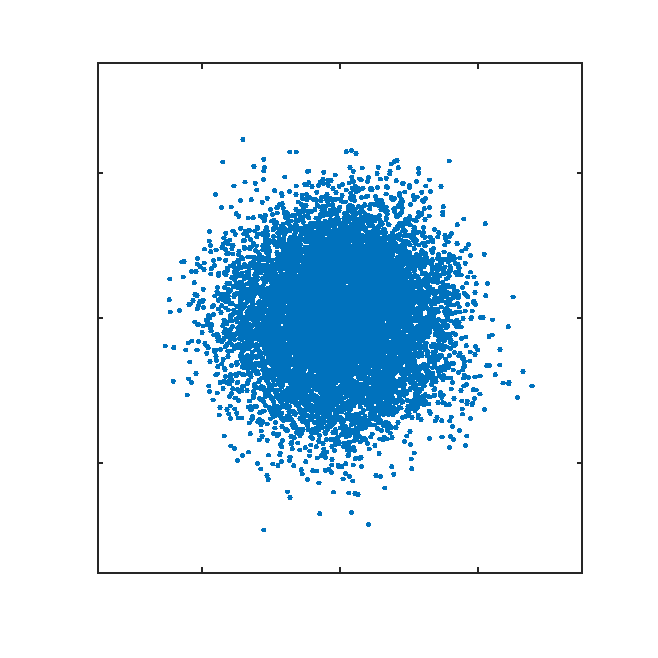
\includegraphics[scale=1]{model19_aux3_z_scatter-inc}
\end{picture}%
\begin{picture}(300,300)(0,0)
\fontsize{6}{0}\selectfont\put(89.0391,28.3198){\makebox(0,0)[t]{\textcolor[rgb]{0.15,0.15,0.15}{{-50}}}}
\fontsize{6}{0}\selectfont\put(155.25,28.3198){\makebox(0,0)[t]{\textcolor[rgb]{0.15,0.15,0.15}{{0}}}}
\fontsize{6}{0}\selectfont\put(221.461,28.3198){\makebox(0,0)[t]{\textcolor[rgb]{0.15,0.15,0.15}{{50}}}}
\fontsize{6}{0}\selectfont\put(35.8804,85.6221){\makebox(0,0)[r]{\textcolor[rgb]{0.15,0.15,0.15}{{-50}}}}
\fontsize{6}{0}\selectfont\put(35.8804,155.25){\makebox(0,0)[r]{\textcolor[rgb]{0.15,0.15,0.15}{{0}}}}
\fontsize{6}{0}\selectfont\put(35.8804,224.878){\makebox(0,0)[r]{\textcolor[rgb]{0.15,0.15,0.15}{{50}}}}
\fontsize{6}{0}\selectfont\put(155.25,287.5){\makebox(0,0)[b]{\textcolor[rgb]{0,0,0}{{Scatter}}}}
\end{picture}
